% GNUPLOT: LaTeX picture with Postscript
\begingroup
  \fontfamily{Serif}%
  \selectfont
  \makeatletter
  \providecommand\color[2][]{%
    \GenericError{(gnuplot) \space\space\space\@spaces}{%
      Package color not loaded in conjunction with
      terminal option `colourtext'%
    }{See the gnuplot documentation for explanation.%
    }{Either use 'blacktext' in gnuplot or load the package
      color.sty in LaTeX.}%
    \renewcommand\color[2][]{}%
  }%
  \providecommand\includegraphics[2][]{%
    \GenericError{(gnuplot) \space\space\space\@spaces}{%
      Package graphicx or graphics not loaded%
    }{See the gnuplot documentation for explanation.%
    }{The gnuplot epslatex terminal needs graphicx.sty or graphics.sty.}%
    \renewcommand\includegraphics[2][]{}%
  }%
  \providecommand\rotatebox[2]{#2}%
  \@ifundefined{ifGPcolor}{%
    \newif\ifGPcolor
    \GPcolortrue
  }{}%
  \@ifundefined{ifGPblacktext}{%
    \newif\ifGPblacktext
    \GPblacktexttrue
  }{}%
  % define a \g@addto@macro without @ in the name:
  \let\gplgaddtomacro\g@addto@macro
  % define empty templates for all commands taking text:
  \gdef\gplbacktext{}%
  \gdef\gplfronttext{}%
  \makeatother
  \ifGPblacktext
    % no textcolor at all
    \def\colorrgb#1{}%
    \def\colorgray#1{}%
  \else
    % gray or color?
    \ifGPcolor
      \def\colorrgb#1{\color[rgb]{#1}}%
      \def\colorgray#1{\color[gray]{#1}}%
      \expandafter\def\csname LTw\endcsname{\color{white}}%
      \expandafter\def\csname LTb\endcsname{\color{black}}%
      \expandafter\def\csname LTa\endcsname{\color{black}}%
      \expandafter\def\csname LT0\endcsname{\color[rgb]{1,0,0}}%
      \expandafter\def\csname LT1\endcsname{\color[rgb]{0,1,0}}%
      \expandafter\def\csname LT2\endcsname{\color[rgb]{0,0,1}}%
      \expandafter\def\csname LT3\endcsname{\color[rgb]{1,0,1}}%
      \expandafter\def\csname LT4\endcsname{\color[rgb]{0,1,1}}%
      \expandafter\def\csname LT5\endcsname{\color[rgb]{1,1,0}}%
      \expandafter\def\csname LT6\endcsname{\color[rgb]{0,0,0}}%
      \expandafter\def\csname LT7\endcsname{\color[rgb]{1,0.3,0}}%
      \expandafter\def\csname LT8\endcsname{\color[rgb]{0.5,0.5,0.5}}%
    \else
      % gray
      \def\colorrgb#1{\color{black}}%
      \def\colorgray#1{\color[gray]{#1}}%
      \expandafter\def\csname LTw\endcsname{\color{white}}%
      \expandafter\def\csname LTb\endcsname{\color{black}}%
      \expandafter\def\csname LTa\endcsname{\color{black}}%
      \expandafter\def\csname LT0\endcsname{\color{black}}%
      \expandafter\def\csname LT1\endcsname{\color{black}}%
      \expandafter\def\csname LT2\endcsname{\color{black}}%
      \expandafter\def\csname LT3\endcsname{\color{black}}%
      \expandafter\def\csname LT4\endcsname{\color{black}}%
      \expandafter\def\csname LT5\endcsname{\color{black}}%
      \expandafter\def\csname LT6\endcsname{\color{black}}%
      \expandafter\def\csname LT7\endcsname{\color{black}}%
      \expandafter\def\csname LT8\endcsname{\color{black}}%
    \fi
  \fi
  \setlength{\unitlength}{0.0500bp}%
  \begin{picture}(12960.00,8640.00)%
    \gplgaddtomacro\gplbacktext{%
      \csname LTb\endcsname%
      \put(980,640){\makebox(0,0)[r]{\strut{} 0}}%
      \csname LTb\endcsname%
      \put(980,1380){\makebox(0,0)[r]{\strut{} 100}}%
      \csname LTb\endcsname%
      \put(980,2120){\makebox(0,0)[r]{\strut{} 200}}%
      \csname LTb\endcsname%
      \put(980,2860){\makebox(0,0)[r]{\strut{} 300}}%
      \csname LTb\endcsname%
      \put(980,3600){\makebox(0,0)[r]{\strut{} 400}}%
      \csname LTb\endcsname%
      \put(980,4340){\makebox(0,0)[r]{\strut{} 500}}%
      \csname LTb\endcsname%
      \put(980,5079){\makebox(0,0)[r]{\strut{} 600}}%
      \csname LTb\endcsname%
      \put(980,5819){\makebox(0,0)[r]{\strut{} 700}}%
      \csname LTb\endcsname%
      \put(980,6559){\makebox(0,0)[r]{\strut{} 800}}%
      \csname LTb\endcsname%
      \put(980,7299){\makebox(0,0)[r]{\strut{} 900}}%
      \csname LTb\endcsname%
      \put(980,8039){\makebox(0,0)[r]{\strut{} 1000}}%
      \csname LTb\endcsname%
      \put(1582,440){\makebox(0,0){\strut{} 1998}}%
      \csname LTb\endcsname%
      \put(2546,440){\makebox(0,0){\strut{} 2000}}%
      \csname LTb\endcsname%
      \put(3511,440){\makebox(0,0){\strut{} 2002}}%
      \csname LTb\endcsname%
      \put(4475,440){\makebox(0,0){\strut{} 2004}}%
      \csname LTb\endcsname%
      \put(5439,440){\makebox(0,0){\strut{} 2006}}%
      \csname LTb\endcsname%
      \put(6403,440){\makebox(0,0){\strut{} 2008}}%
      \csname LTb\endcsname%
      \put(7368,440){\makebox(0,0){\strut{} 2010}}%
      \csname LTb\endcsname%
      \put(8332,440){\makebox(0,0){\strut{} 2012}}%
      \csname LTb\endcsname%
      \put(9296,440){\makebox(0,0){\strut{} 2014}}%
      \put(160,4339){\rotatebox{-270}{\makebox(0,0){\strut{}Gross Earnings (per annum, GBP $\pounds$, not adjusted)}}}%
      \put(5198,040){\makebox(0,0){\strut{}Year}}%
      \put(5198,8639){\makebox(0,0){\strut{}Employee Earnings, Percentiles}}%
      \put(5198,8339){\makebox(0,0){\strut{}(Tenth--, $25\%$, $50\%$, $75\%$ and Nintieth-- Percentile Boundaries)}}%
      \put(9600,3200){\makebox(0,0)[l]{\strut{}\small UK Employee Earnings, Percentiles}}%
      \put(9600,2100){\makebox(0,0)[l]{\strut{}\begin{minipage}[t][][t]{6.3cm}\small
UK employee earnings (gross) per annum, not adjusted, tenth-- / $25\%$ / $50\%$ / $75\%$ and nintieth-- percentiles. Based on full--time and part--time employees receiving adult rates of pay. Source: {\it Distribution of gross weekly pay, United Kingdom, April 1997--2014}, {\it Annual Survey of Hours and Earnings (ASHE)}, \textit{\it ONS}.
\end{minipage}}}%
    }%
    \gplgaddtomacro\gplfronttext{%
      \csname LTb\endcsname%
      \put(12056,7889){\makebox(0,0)[r]{\strut{}$10\%$ Earned Less Than}}%
      \csname LTb\endcsname%
      \put(12056,7589){\makebox(0,0)[r]{\strut{}$25\%$ Earned Less Than}}%
      \csname LTb\endcsname%
      \put(12056,7289){\makebox(0,0)[r]{\strut{}$50\%$ Earned Less Than}}%
      \csname LTb\endcsname%
      \put(12056,6989){\makebox(0,0)[r]{\strut{}$75\%$ Earned Less Than}}%
      \csname LTb\endcsname%
      \put(12056,6689){\makebox(0,0)[r]{\strut{}$90\%$ Earned Less Than}}%
    }%
    \gplbacktext
    \put(0,0){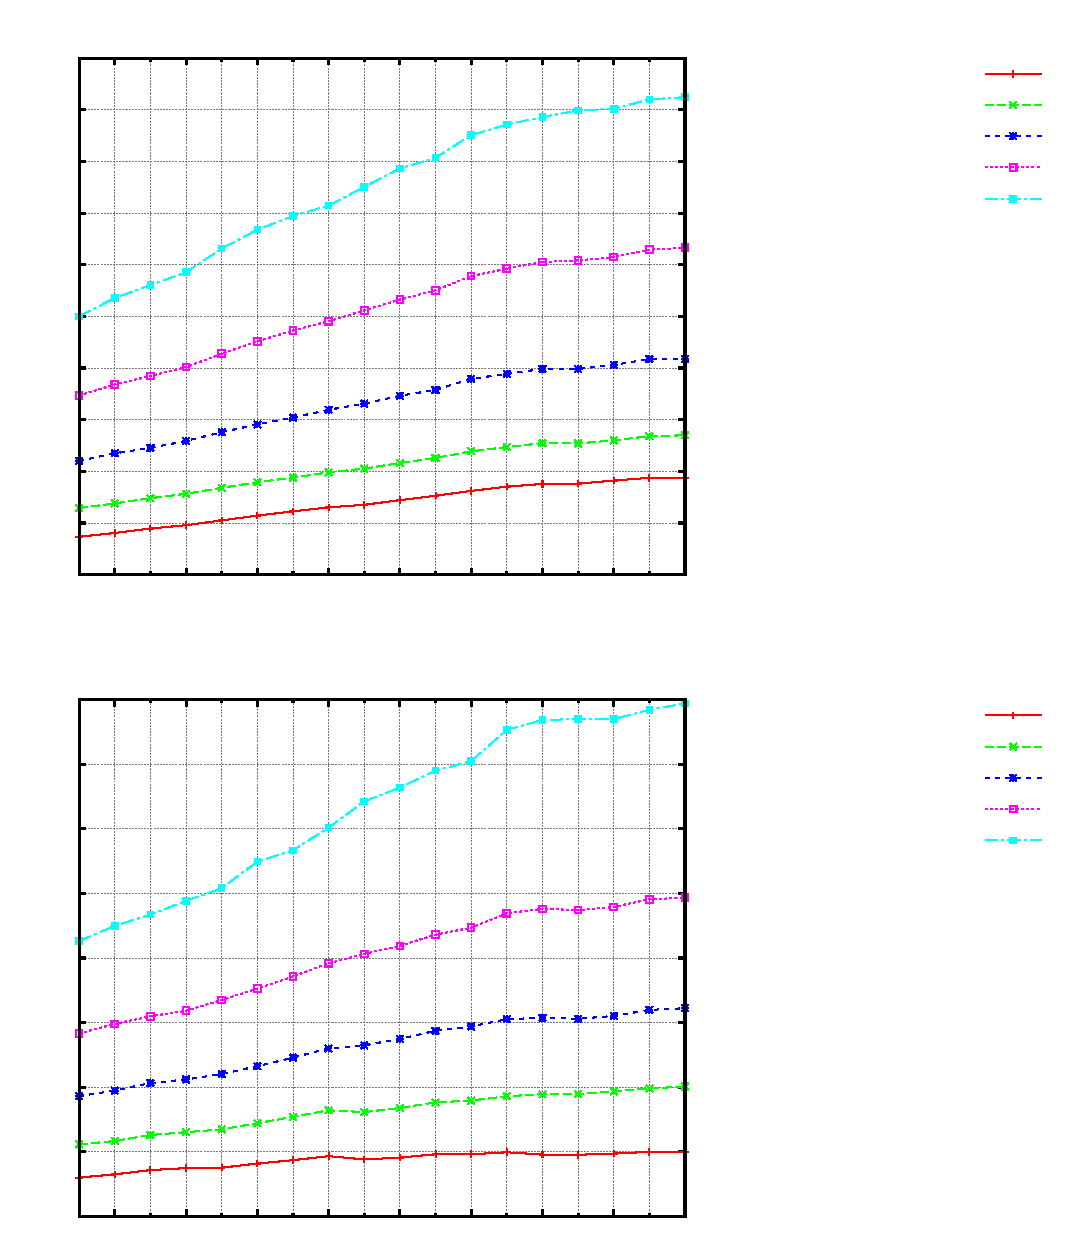
\includegraphics{./plots/wage-percentiles-all/wage-percentiles.eps}}%
    \gplfronttext
  \end{picture}%
\endgroup
